\documentclass[12pt]{article}
% This work is about rootkits
\usepackage[T2A]{fontenc}
\usepackage[utf8]{inputenc}
\usepackage{multicol}
\usepackage{gensymb}
\usepackage{graphicx}
\usepackage{listings}
\usepackage{verbatim}

\title{Kernel rootkits in Linux: low-level approach and prevention}
\date{}
\author{Ivan Galinskiy}

\begin{document}
  \maketitle
  
  \section{Kinds of rootkits}
  \subsection{Classification}
  What exactly are the rootkits? In the malware classification, rootkits are
  programs designed to hide the fact of system intrusion by hiding processes,
  users, files etc. This is the base classification, which is true for all
  kinds of rootkits. But if we look at real samples, deviations appear. For
  example, in some cases the rootkit is not just ``standalone'', but a part of
  another piece of malware which is being hidden. A very good example is
  Rustock.C designed for Windows.

  \subsection{Basic principles of work}
  Obviously, the process of hiding something is based on modifying system
  ``internals'', requiring thus some way to gain administrative (root)
  privileges. This can be done in very different ways, and besides, it is not
  part of rootkit's job, so we will skip that. But there are basically two
  ways the rootkit ``holds'' itself on the main system:
  \begin{enumerate}
    \item Modifying files on the filesystem. When a program has administrative
      rights on the target machine, it can (almost always) do whatever it
      ``wants''. For example, modifying the passwd or sudo utilities will
      probably get users' passwords. The disadvantages are obvious. To detect
      the rootkit, the user needs to check main utilities' checksums from a
      trusted operating system (either by loading with LiveCD or by taking the
      harddisk to another machine).

    \item Modifying only the RAM. Of course, at first sight it may look a bit
      strange, as with a reboot anything will return to normal. But just
      imagine a server with, lets say, 2 years uptime? Now it looks better,
      and this kind of rootkits is much tougher (and more interesting to
      research).
  \end{enumerate}

  \section{A brief look at DR Linux rootkit}
  
  Well, finding this one was not a difficult task. Besides, it's one of the
  most up-to-date open-source rootkits available. Others are either very old,
  or don't match our context, so we will not look at them. The source code
  indicates that this rootkit is based on debug registers. According to Intel
  documentation, the debugging registers are DR0 - DR7. DR0 - DR3 registers
  hold four linear addresses. DR4 and DR5 are reserved for extended debugging
  and we are not going to look at them now. DR6 is the ``Debug State
  Register'' and DR7 is the ``Debug Control Register''. What is their purpose?
  The below scheme from Intel documentation explains some things.
  \begin{figure}[h]
    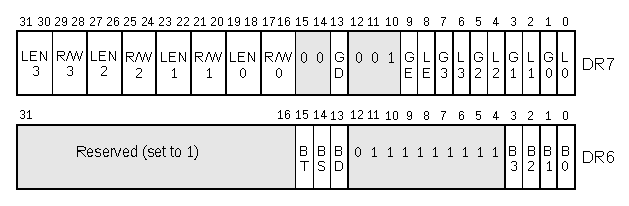
\includegraphics[width=\linewidth, keepaspectratio]{dregs}
  \end{figure}
  The one interesting is the DR7, which controls the debugging behaviour. For
  the rootkit, the usefullness is in the ability to control read, write or
  execute operations (or their combinations) on the breakpoints (note: the
  settings are individual for each breakpoint). Obviously, the breakpoints are
  not useful by themselves. When a breakpoint is reached, after executing it,
  the processor emits a \verb!#DB! exception, which is catched by the kernel
  handler in normal cases. But the rootkit changes the handler in Interrupt
  Descriptor Table to its own (saving the previous).

  \section{Interception techniques}

  Wait, is this the only way to control system internals? Actually, more
  methods were created through the time, but all them are based on modifying
  well-known system structures, the quantity of which is not so big. What
  structures? Some of them are IDT, MSR, DR registers (as seen
  above), syscall tables... What are all these abbreviatures? They may look
  scary at first sight, but the things are simpler. So what all those things do?

  \begin{itemize}
    \item IDT means Interrupt Descriptor Table. In simple words, it contains
      addresses of handlers for interrupts. As we have seen in the DR rootkit,
      it may be very useful. There is also another detail.  Before Pentium II
      was introduced, system calls (i.e. calls from user applications to
      kernel) were performed using the \verb!0x80!  interrupt (loading the
      system call number into EAX register before invoking interrupt). And
      guess what? The handler for that interrupt was stored in IDT too.

    \item MSR stands for Model Specific Registers. As I already told, before
      Pentium II, interrupts were used to make system calls. It's a simple
      way, but unfortunately, slow. That's when \verb!SYSENTER/SYSCALL! and
      \verb!SYSEXIT/SYSRET! (for Intel/AMD respectively) commands were
      introduced, providing a faster way to make system calls. Now the handler
      of the call was not in IDT, but in a set of MSR registers. They store
      the target instruction, stack segment pointer etc. But the most
      interesting and useful for us is the \verb!IA_32_SYSENTER_EIP! which
      stores the target instruction. Changing it to something else will
      redirect all the system calls into the new procedure.

    \item So what is the difference between the above two methods? Only the
      way to \emph{call} system procedures! Even if we examine the source of
      \verb!ia32_sysenter_target! (there is where \verb!IA_32_SYSENTER_EIP!
  points by default), we find
  ``\verb!call *ia32_sys_call_table(,%rax,8)!''. This means that those
  procedures are the same in both cases (it would be strange otherwise). And,
  of course, modifying pointers in this table can be very funny for the
  rootkit (and more for the machine owner).
  \end{itemize}


  \subsection{Modifying IDT}
  There are some other ways, of course, but now we will concentrate on the
  ones listed above and try to perform these ``tricks''. So, the first in the
  list is interception of interrupts via IDT. Ok, let's begin.
  \begin{itemize}
    \item First of all, I am going to be as kernel version independent as I
      can. It means that I am going to use resources available in the
      processor rather that predefined macros or whatever.
    \item OK, before we make any changes to IDT, we obviously need to know
      where exactly it resides. An assembly command \verb!SIDT! can help us
      with this, getting the IDTR register contents. In 32-bit systems, IDTR
      contains two fields: the 16-bit limit, specifying the size of the table,
      and 32-bit address which is the location of IDT. But there is a detail
      that led me to mistakes: the address is stored with low-order bytes
      first! We can define a function to get the register contents in
      easily-readable form: \verbatiminput{sidt.h}

    \item Half of the job is done now. However, we still need to get a
      particular entry in the IDT (to store the original interrupt handler,
      for example). In Linux on 32-bit systems, each entry in IDT is 8-bytes
      long and consists of an offset to the handler and some attributes. The
      funny thing is the offset is not continuous in the entry! The first 16
      bits begin at bit 0 of the IDT entry, and the last 16 are at the end of
      the entry. Tricky, right? The following code can handle with this:
      \verbatiminput{idt.h}

    \item Very good! Now that we have the entries, many things can be
      done. But let's stop with IDT hooking and continue to the next method.
  \end{itemize}

  \subsection{SYSENTER/SYSCALL interception}
  Well, this one is a juicy one! As I already told, beginning with Pentium II,
  Intel processors implemented the new \verb!SYSENTER!/\verb!SYSEXIT!
  instructions (and AMD used \verb!SYSCALL!/\verb!SYSRET!). They decreased the
  overhead of switching from user mode and vice-versa (the interrupts are
  slow). These instructions used special MSR registers to know where the
  target procedure was located. There is one that is specially relevant to us:
  \verb!SYSENTER_EIP_MSR!. Its contents are loaded to the EIP register
  (basically a jump) at the end of \verb!SYSENTER! execution. Initially it
  points to a kernel procedure, but we can change it to our procedure. How can
  it be done?
  \begin{itemize}
    \item First, of course, we need a way to access the
      \verb!SYSENTER_EIP_MSR! register. It's not accessed like the, let's say,
      EAX register. There is a special instruction, \verb!RDMSR!, that does
      it. The only requirement is that the number of MSR register should be
      loaded into ECX (the number of \verb!SYSENTER_EIP_MSR! is 0x176). The
      contents are stored in EDX and EAX registers (EDX is 0 on 32-bit
      systems).
      
    \item Now we can put a new value to the register. This process is
      basically an inverted version of the previous. We load the new value
      into EDX:EAX (EDX is zero, EAX is the new procedure pointer), the MSR
      register number into ECX, and perform the instruction \verb!WRMSR!.
  
    \item I thought that an example would be more helpful than a dry
      description, so here is a sample kernel module for this task (the
      includes were (duh) excluded). It's a kernel module because \verb!WRMSR!
  can only be performed at ring 0:
  \verbatiminput{msr.h}
  \item Obviously, this module doesn't do anything special, it's more like a
    ``proof-of-concept''. But the payload will come later.
  \end{itemize}
\end{document}
